\documentclass[11pt,a4j]{jarticle}
\usepackage[dvipdfmx]{graphicx,color}
\usepackage{wrapfig}
\usepackage{amssymb}
\setlength{\topmargin}{-1.5cm}
\setlength{\textwidth}{15.5cm}
\setlength{\textheight}{25.2cm}
\newlength{\minitwocolumn}
\setlength{\minitwocolumn}{0.5\textwidth}
\addtolength{\minitwocolumn}{-\columnsep}
%\addtolength{\baselineskip}{-0.1\baselineskip}
%
\def\Mmaru#1{{\ooalign{\hfil#1\/\hfil\crcr
\raise.167ex\hbox{\mathhexbox 20D}}}}
%
\begin{document}
\newcommand{\fat}[1]{\mbox{\boldmath $#1$}}
\newcommand{\D}{\partial}
\newcommand{\w}{\omega}
\newcommand{\ga}{\alpha}
\newcommand{\gb}{\beta}
\newcommand{\gx}{\xi}
\newcommand{\gz}{\zeta}
\newcommand{\vhat}[1]{\hat{\fat{#1}}}
\newcommand{\spc}{\vspace{0.7\baselineskip}}
\newcommand{\halfspc}{\vspace{0.3\baselineskip}}
\bibliographystyle{unsrt}
\pagestyle{empty}
\newcommand{\twofig}[2]
 {
   \begin{figure}[h]
     \begin{minipage}[t]{\minitwocolumn}
         \begin{center}   #1
         \end{center}
     \end{minipage}
         \hspace{\columnsep}
     \begin{minipage}[t]{\minitwocolumn}
         \begin{center} #2
         \end{center}
     \end{minipage}
   \end{figure}
 }
%%%%%%%%%%%%%%%%%%%%%%%%%%%%%%%%%
%\vspace*{\baselineskip}
\begin{center}
{\Large \bf 令和1年度 共同研究報告書}
\end{center}
\vspace{2mm}
\begin{center}
{\LARGE \bf 
メソスケールシミュレーションによる緩衝材の特性評価に関する研究} 
\end{center}
\begin{center}
岡山大学環境生命科学研究科\\
木本和志
\end{center}
\vspace{10mm}
%%%%%%%%%%%%%%%%%%%%%%%%%%%%%%%%%%%%%%%%%%%%%%%%%%%%%%%%%%%%%%%%
\section{はじめに}
高レベル放射性廃棄物(HLW)の地層処分において、ベントナイト緩衝材は、地下水と放射性各種の移行を抑制する役割を長期に渡って果たすことが求められる。ベントナイト粘土の主成分であるモンモリロナイトは、ナノスケールの微細な間隙をもつ多孔質構造を作り、熱や物質輸送特性は間隙の構造や水分の分布や移動によっても変化する。例えば、積層した粘土層間では粘土表面に間隙水が強く水和されており、水分移動が起こりにくく、積層した粘土間に残されたより大きな間隙中にあるバルク水は比較的移動しやすいと考えられる。これらが粘土緩衝材のスケールでどのような透水性となって現れるかは、間隙率や飽和度だけでなく、間隙の幾何構造や間隙径の分布に影響されることは明らかで、従って、粘土含水系における水分の分布や間隙の幾何学的形状やスケールについて理解することは、透水性や物質輸送特性の正確な評価を行う上で重要である。しかしながら、粘土含水系のナノスケールでの粘土鉱物や間隙、間隙水の状態を顕微鏡下で直接観察することは難しく、これら微視的な多孔質構造に関する正確な理解はあまり進んでいない。

粘土鉱物の結晶構造や水和および膨潤挙動については、分子動力(MD)学法に基づくシミューレション解析が精力的に行われてきた。MD法では、物質を構成する原子や分子間の相互作用則を与える他、系の性質を仮定することなく粘性や拡散係数、誘電率といったマクロ物性を評価することができる。しかしながら、構成原子全ての自由度を考慮する全原子MDは計算負荷が非常に高く、取り扱うことのできるモデルの時空間的スケールは概ねナノメートル、ナノ秒の範囲である。従って、多数の粘土分子から構成される系を全原子MD計算で解析することは、現状では困難である。これに対して著者らは、粗視化分子動力学の方法を用い、ナノからマイクロメートルスケールでの、粘土含水系の挙動を調べることを目的とした数値シミュレーション技術の開発に取り組んで来た。このような空間スケールは、連続体近似が可能なmm程度のスケールと、分子シミュレーションが必要となるナノスケールの中間に当たることから、粗視化MDの方法をメソスケールMD(メソMD)と称している。メソMDでは、物質を構成する原子のうち、相対位置を大きく変化させることなく運動すると予想される原子のグループを、一つの仮想的な粒子(粗視化粒子)で表現することで、モデルの自由度を削減する。これにより、より大きなスケールで物質をモデル化しその挙動を計算機シミュレーションによって調べることを可能にする。

著者らが開発を行っている粘土含水系のメソMDシミュレーションでは、粘土結晶の単位構造と、そこに水和された間隙水を一つの粗視化粒子で表し、粗視化粒子間の相互作用力は全原子MD計算の結果から与えている。この方法により、指定された温度、圧力で圧縮したときに生じる粘土含水系の凝集挙動を調べている。また、メソMD解析で得られた粘土含水系の組織構造モデルを用いて拡散や変形解析を行い、微視的な多孔質構造を考慮したマクロ拡散係数や弾性係数の評価が可能であることを示してきた。また、粘土分子同士が接近しているときには、近接する粗視化粒子間で水分の移動を許容することで、不自然な気泡を残すことなく、安定した組織構造が得られることも昨年度までの研究によって明らかとすることができた。一方で、メソMD解析の結果として得られた組織構造が、特定のシミュレーション条件において有意に変化したかを判定し、組織構造の形成に与える重要な因子を特定することは未だ実現できていない。また、メソMDメソ計算により、拡散係数などのマクロ物性が組織構造のどのような特徴を反映して決まるかといった点を理解する方法も明らかとなっていない。
これらの問題は、シミュレーション結果の妥当性の検証や、マクロ物性に強い影響を与える因子の特定と定量化、ひいては、マクロ物性の発現メカニズムを理解する上で解決すべく残された課題となっている。

以上を踏まえ、本年度は、メソMD計算で得られた組織構造を解析し、定量的に特徴づける方法の開発と実装を目的として研究を行った。具体的には、メソMDシミュレーションの結果から、X線回折パターンや動径分布関数を合成することで、粘土分子の平均的な積総数や層間距離を評価することを可能とする。これらは、実測可能かつ、物理的な意味が明確なものであるため、粘土含水系の積層構造形成メカニズムの理解や影響因子の抽出と序列、計算モデルの妥当性の検証が可能となる。また、シミューレションで得られた組織構造の局所密度を評価ならびに可視化することで、層間と層外の間隙を区別する方法を提案する。これは、今後、物質輸送に与える組織構造の影響を調べる際に必要となる技術と考えられる。
%これにより、メソMD計算の結果が、計算条件によって有意に変化下かどうかを判定することや、計算結果として得られる組織構造の成因を理解するために有用な情報を得ること、

以下では、上記の組織構造解析を行うために用意した、2種類の粘土含水系のモデルを次節に置いて示す。続いて、フーリエ変換を利用したX線回折パターンの合成方法、粘土の積層数を評価するために考案した動径分布関数と、メソスケール間隙を抽出するための局所密度の定義時計方法を順に述べる。これら一連のプロットを、メソMD計算結果から実際に計算して示し、そこから読み取ることができる情報について述べる。最後に、2種類メソMDモデル対して得られる組織構造の特徴量を比較することで、メソMDの計算条件が組織構造のどのような特徴の差として現れるかを議論する。


\section{メソMD計算モデル}
%--------------------
\subsection{粘土含水系モデルとメソMDシミューレションの条件}
本研究において組織構造解析に用いる2種類の粘土含水系メソMDモデル(モデル1と2)を
図\ref{fig:fig1}と図\ref{fig:fig2}示す。
これらの図は、粘土分子の初期状態(時刻$t=0$)における分布と、 粘土分子幅(粒径)のヒストグラムを示している。
いずれのモデルも周期構造を仮定し,粘土分子の初期配置を示した図には,
周期構造のユニットセルが破線で示されている.
2つのモデルの主たる違いは、粒径分布にありそれぞれのモデル分子数と粒径は
正規分布によって以下のように設定している。
\begin{itemize}
\item
モデル1
	\begin{itemize}
		\item 粘土分子数: 80
		\item 粗視化粒子数: 3,194
		\item 平均粒径 (標準偏差): 40 (10)[{\rm nm}]
	\end{itemize}
\item
モデル2
	\begin{itemize}
		\item 粘土分子数: 80
		\item 粗視化粒子数: 3,237
		\item 平均粒径 (標準偏差): 50(27)[{\rm nm}]
	\end{itemize}
\end{itemize}
これらの数値から明らかなように、モデル2はモデル1に比べて粒径分布の分散が大きく設定されている。
初期状態でのユニットセルのサイズは、200$\times$200[nm]の正方形とし、1[ns]の間にユニットセルを
等方的に65\%圧縮する。その結果、最終的には70$\times$70[nm]の正方形ユニットセルに、約80の粘土分子が
充填された組織構造が得られる。
なお、粘土分子は全て初期状態では二層膨潤に相当する水和水を持つものとする。ただし、
圧縮の過程において、近接する粗視化粒子間では粒子径のポテンシャルエネルギーが下がる場合には、
水和水の移動が生じることを許容するモデルを用いる。そのため、最終的にえられた組織構造において、水分
分布は一様でなく、必ずしも平均的に二層膨潤状態が維持される保証はない。圧縮は等温条件で進め、
系の温度は,粗視化粒子の運動エネルギーを各時間ステップでスケーリングすることで一定値を保つように
制御した.
%--------------------
\begin{figure}[h]
	\begin{center}
	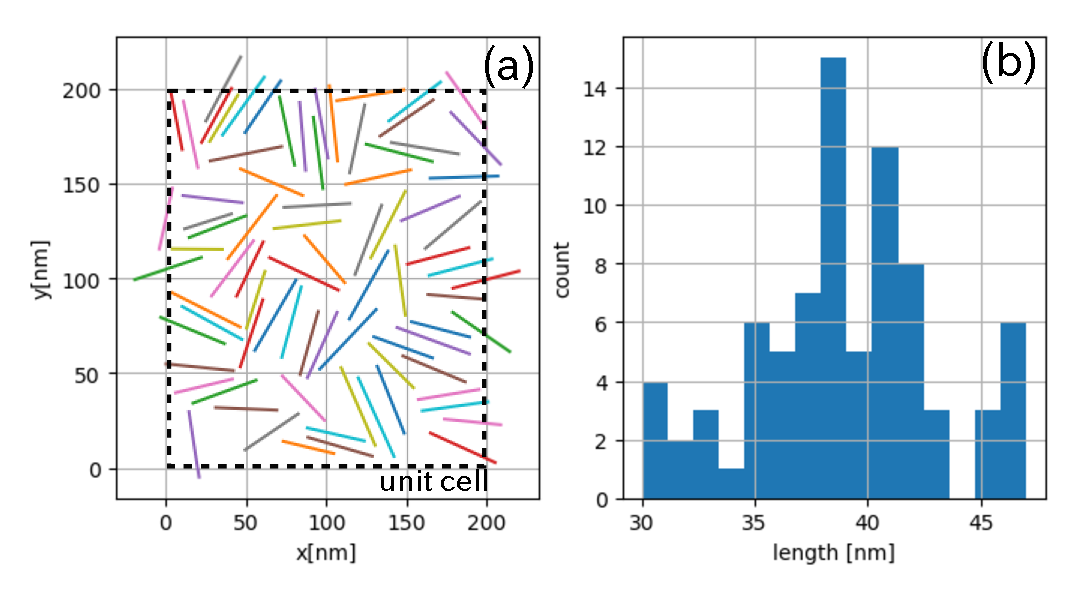
\includegraphics[width=0.8\linewidth]{Figs/fig1.eps} 
	\end{center}
	\caption{
		メソスケールMD解析モデル1. (a)粘土分子の初期分布.(b)粘土分子幅のヒストグラム. 
	} 
	\label{fig:fig1}
\end{figure}
%--------------------
\begin{figure}[h]
	\begin{center}
	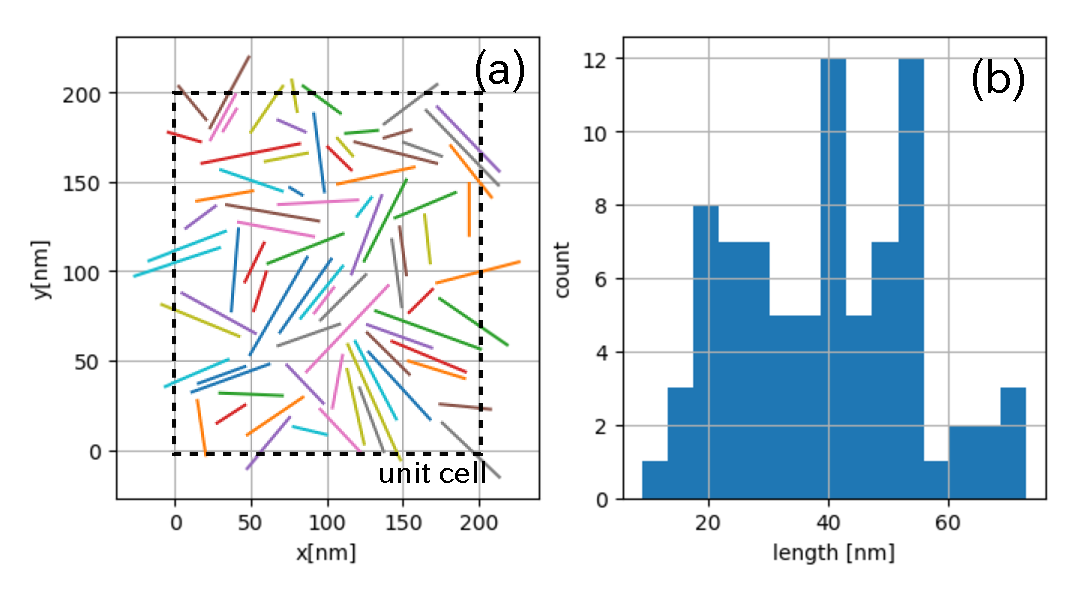
\includegraphics[width=0.8\linewidth]{Figs/fig2.eps} 
	\end{center}
	\caption{
		メソスケールMD解析モデル2. (a)粘土分子の初期分布.(b)粘土分子幅のヒストグラム. 
	} 
	\label{fig:fig2}
\end{figure}
%--------------------
\subsection{圧縮凝集過程のシミュレーション結果}
図\ref{fig:fig3}と図\ref{fig:fig4}に,上記のモデルと計算条件で行ったメソMD解析の結果を示す。
これらの図は、粘土分子分布のスナップショットを0.2ns毎に示したもので,ユニットセルの等温圧縮に
よる粘土分子の凝集挙動を示している。いずれのモデルでも、比較的早い段階から、近接する粘土分子が
積層構造を作るが、積総数はあまり大きくならない。また、積層した分子の間に残された大きな間隙が、
ユニットセルの圧縮に伴い、次第に縮小されて最終的にはほとんど消失する様子が見られる。
これらの結果では、2つのモデルにおいて粘土分子の配置は途中段階でも圧縮終了後も当然互いに異なるが、
凝集挙動や最終的にえられた組織構造に本質的な差があるかどうかは明らかでない。
しかしながら、このようにして得られた組織構造を次節で述べる方法によって処理し、X線回折パターン等の形で
比較すると、2つの組織構造モデルには有意な差があることが明らかとなる。
\begin{figure}[h]
	\begin{center}
	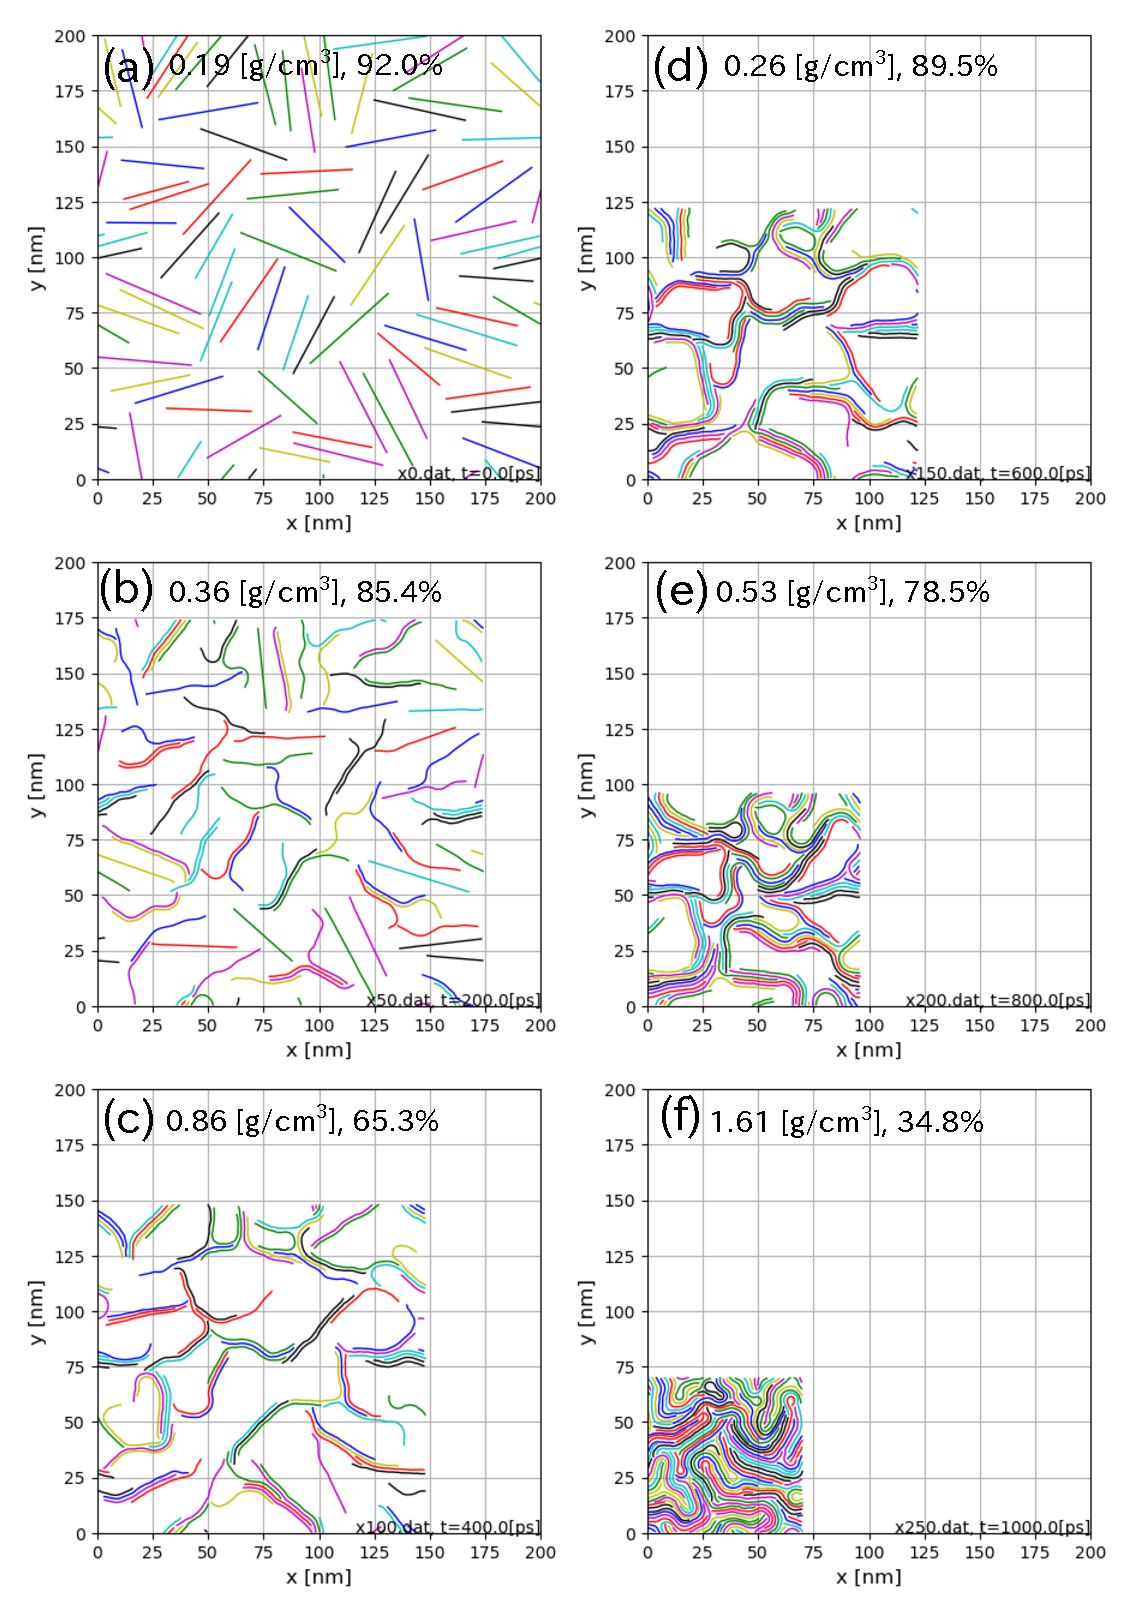
\includegraphics[width=1.0\linewidth]{Figs/fig3.eps} 
	\end{center}
	\caption{
		ユニットセルの圧縮に伴う粘土分子の凝集挙動(モデル1).
	} 
	\label{fig:fig3}
\end{figure}
%--------------------
\begin{figure}[h]
	\begin{center}
	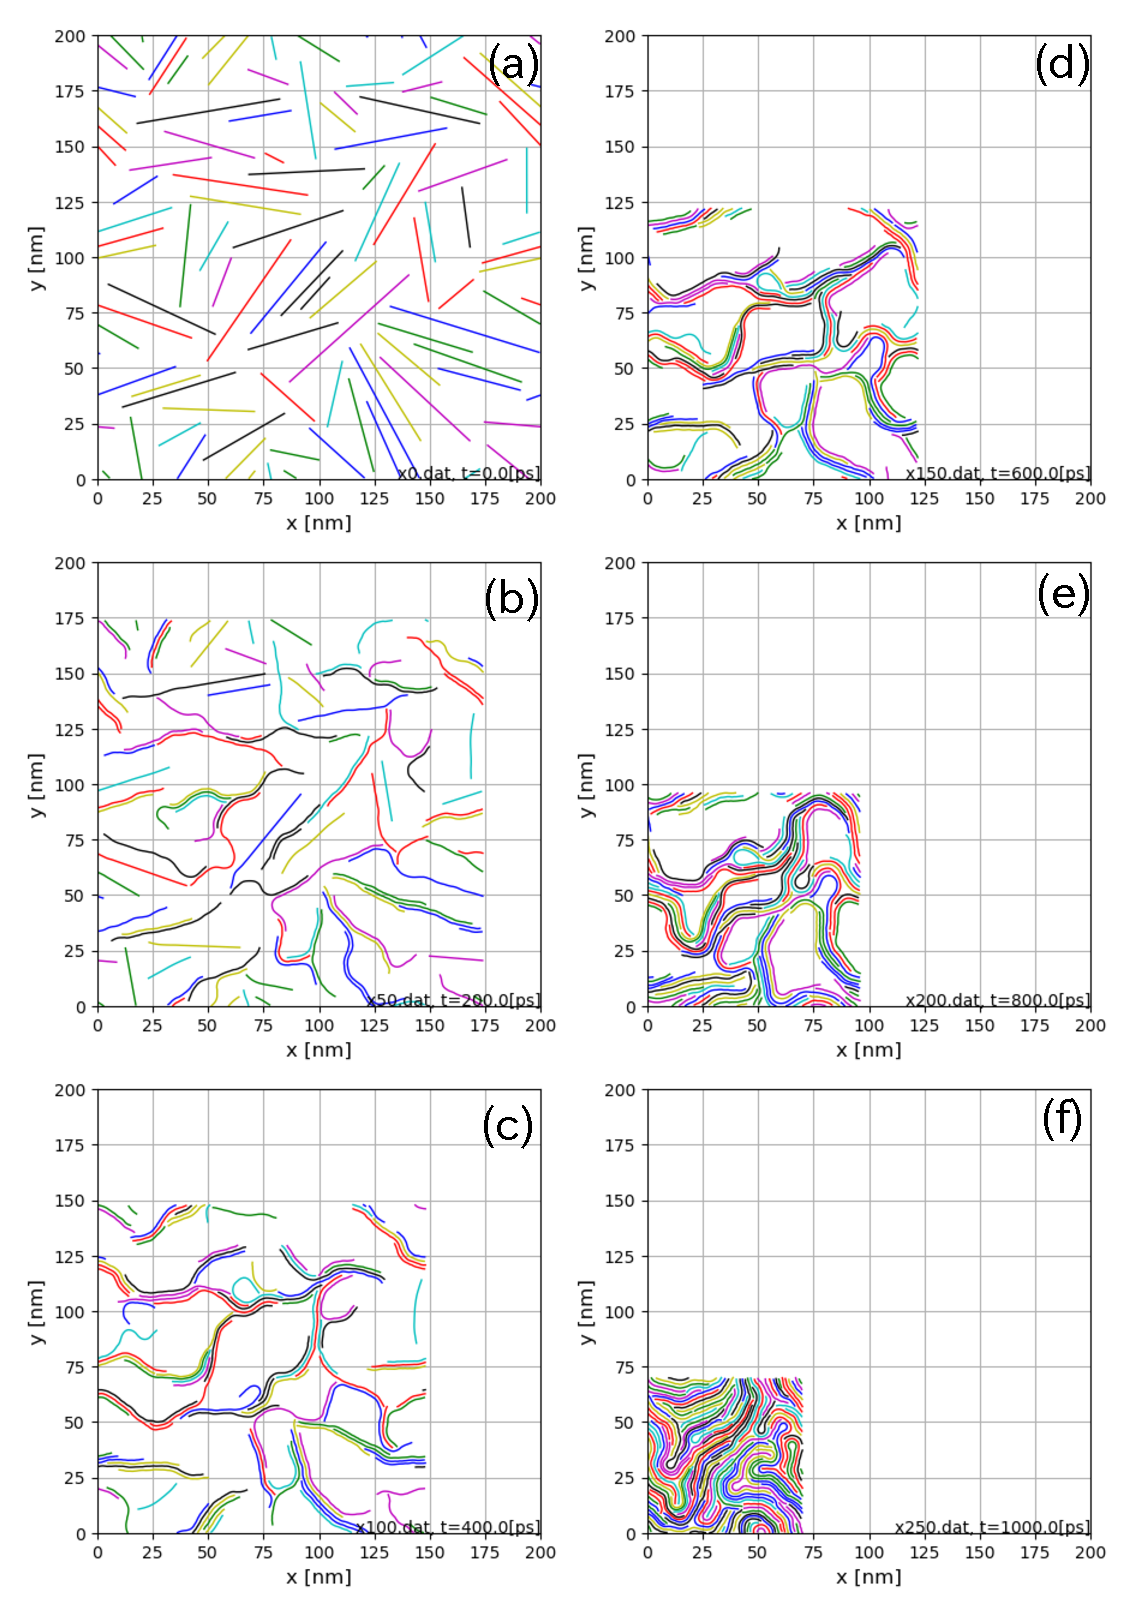
\includegraphics[width=1.0\linewidth]{Figs/fig4.eps} 
	\end{center}
	\caption{
		ユニットセルの圧縮に伴う粘土分子の凝集挙動(モデル2).
	} 
	\label{fig:fig4}
\end{figure}
%--------------------

\section{組織構造解析の方法と計算例}
メソMD解析の結果として得られた組織構造を,定量的に特徴づけるために次の4つの分布を求める。
\begin{itemize}
	\item X線回折(X-ray diffraction:XRD)パターン
	\item 動径分布関数(Radial distribution function:RDF)
	\item 局所密度分布
	\item 粗視化粒子方向の確率密度分布
\end{itemize}
以下、これらの分布関数の定義と求め方を示すとともに,モデル1について実際に計算した
4種類の分布関数とそこから読み取ることのできる情報について述べる.
\subsection{X線回折(XRD)パターン}
試料によって散乱されたX線の観測方向による散乱X線強度の変化をプロットしたグラフを
X線回折パターンと呼ぶ.X線源がmonochromaticな平面波を試料に照射していると仮定するとき、
位置$\fat{x}$における入射X線$u(\fat{x})$は波数ベクトル$\fat{k}^{in}$を用いて
\begin{equation}
	u^{in}(\fat{x})=I_0 \exp(i\fat{k}^{in}\cdot\fat{x})
	\label{eqn:uin}
\end{equation}
と表すことができる。今、試料を構成する物質の作る電荷密度分布を$\rho(\fat{x})$、
散乱X線の波数ベクトルを$\fat{k}_{sc}$とすれば、無限遠方での散乱X線を
\begin{equation}
	u^{sc}(2\theta)=I_0 \int \rho(\fat{x})\exp(i\fat{k}\cdot\fat{x})d\fat{x}, \ \ 
	\left(\fat{k}=\fat{k}^{sc}-\fat{k}^{in}\right)
	\label{eqn:usc}
\end{equation}
と表すことができる。
ただし$2\theta$は$\fat{k}^{in}$と$\fat{k}^{sc}$が成す角を表す.
X線計測で実際に測定することができるのはX線強度だけである.
散乱X線の強度は式(\ref{eqn:usc})の絶対値をとり$\left| u^{sc}(\fat{x})\right|$で,
与えられ,
\begin{equation}
	\left|u(2\theta)\right|
	=
	\left|\int \rho(\fat{x}) \exp(i\fat{k}\cdot \fat{x}) d\fat{x} \right|
	\label{eqn:I2th_bar}
\end{equation}
と書くことができる。この量は,入射X線の伝播方向を$\varphi$にも依存するので,
\begin{equation}
	I_\varphi(2\theta):
		=\frac{\left|u(2\theta)\right|}{I_0}
		=
	\left|\int \rho(\fat{x}) \exp(i\fat{k}\cdot \fat{x}) d\fat{x} \right|
	\label{eqn:Iphi}
\end{equation}
と表すことにする.実際には試料は様々な方向を向いていると考えれば、試料からみて
X線はあらゆる方向から入射されることになる。その時観測される散乱X線強度$I(2\theta)$は
式(\ref{eqn:Iphi})を$\varphi$について積分した
\begin{equation}
	I(2\theta)=\int I_{\varphi}(2\theta) d\varphi
	\label{eqn:XRD}
\end{equation}
で与えられることが分かる.式(\ref{eqn:XRD})を角度$2\theta$の関数として表したものが
X線回折パターンであると考えることができる。
従って,メソMDで得られた組織構造から電荷分布を決定し,式(\ref{eqn:Iphi})と式(\ref{eqn:XRD})
を求めれば、シミュレーション結果に対応したXRDパターンを合成することができる。
このとき,式(\ref{eqn:Iphi})の積分は電荷密度分布のフーリエ変換を計算することによって評価する
ことができる。
本研究では、電荷密度$\rho(\fat{x})$の最も簡単なモデルとして,
固相領域を表す次のような特性関数$\Gamma(\fat{x})$を用いる
\begin{equation}
	\Gamma(\fat{x})=\left\{
		\begin{array}{cc}
			1 &  \fat{x} \in D_s \\
			0 &  otherwise
		\end{array}
	\right.
	\label{eqn:Gamma}
\end{equation}
ただし$D_s$は組織構造モデルにおいて粘土分子が占める固相領域を意味する.
このモデルでは,電荷は粘土分子内で均一に分布しており、粘土分子内の電荷分布による
散乱の指向性や、水和水によるX線の散乱の影響ともに無視されている。
しかしながら、間隙水による散乱の影響は電荷量から考えて粘土分子による散乱よりも影響が小さいと考えられる。
また、粘土分子の内部構造に起因した散乱パターンは、観測方向$2\theta$が比較的大きな範囲に現れるため、
ここで興味の対象となる、粘土分子の積層構造に起因した回折ピークの位置や強度には影響がない。
以上のことからから粘土分子の内部構造や間隙水分布を無視した電荷分布を用いても、
粘土の積層構造や膨潤状態を調べるためXRDパターンの合成において支障はないと言える。
なお、メソMD結果からXRDパターンを合成する際には、特性関数$\Gamma(\fat{x})$を適当な空間解像度で
ピクセル画像として構成する。その空間変数に関する2次元フーリエ変換を離散フーリエ変換によって
計算すれば、全ての波数ベクトル$\fat{k}$に対して式(\ref{eqn:Iphi})右辺を得ることができる。
波数ベクトル$\fat{k}$の方向$2\theta$に応じて計算されたフーリエスペクトルを
サンプリングすれば、各$\theta$に対する$I_\varphi(2\theta)$を得ることができる。
波数空間におけるこのようなサンプリングを入射方向$\varphi$を変えて行い、その結果を
加算すれば、XRD試験で観測される回折パターン$I(2\theta)$を合成することができる。
%%%%%%%%%
% XRD pattern example, Binary pixel image & 2D FFT
%%%%%%%%
\subsection{動径分布関数}
動径分布関数(radial distribution function: RDF)は、
着目粒子から一定の距離だけ離れた位置に存在する粒子数を表すものである。
正確には、ある粒子を原点として測った動径距離$r$について,
区間$[r,\Delta r)$に位置する粒子の数を$g(r,r+\Delta r)$とするとき、
2次元空間における動径分布関数$f(r)$は
\begin{equation}
	f(r):=\frac{g(r,r+\Delta r)}{2\pi r}
	\label{eqn:RDF}
\end{equation}
で与えられる.
ここで、第$i$番目の粗視化粒子の位置を$\fat{r}_i$とし、区間$[r,r+\Delta r)$で
1,そのほかの位置では0をとる矩形関数を
\begin{equation}
	U(r;\Delta r):=\left\{
		\begin{array}{cc}
			1 &  r \in [r;r+\Delta r)\\
			0 &  otherwise
		\end{array}
	\right.
	\label{eqn:}
\end{equation}
と表すと、$g(r,r+\Delta r)$は$U(r;\Delta r)$を用いて次のように書くことができる。
\begin{equation}
	g(r,\,r+\Delta r)=\sum_{i\neq j} U(r_{ij}-r;\Delta r)
	\label{eqn:gr}
\end{equation}
ただし、
\begin{equation}
	r_{ij}=\left|\fat{r}_i-\fat{r}_j\right|
	\label{eqn:rij}
\end{equation}
とする。式(\ref{eqn:RDF})で定義されるRDFを、組織構造解析にそのまま用いると、粘土分子を構成する
粗視化粒子の規則的な配列に起因した顕著なピークが現れ、粘土分子の積層構造の形成に関する情報を読みとることができない。
%%
%% RDF失敗例
%%
そこで、積層構造に寄与する粗視化分子が優先的にカウントされるように、RDFの定義を以下のように修正する。

粗視化粒子$i$から粒子$j$を望む方向を指す単位ベクトルを
\begin{equation}
	\hat{\fat{r}}_{ij}=\frac{\fat{r}_j-\fat{r}_i}{r_{ij}}
	\label{eqn:rhat}
\end{equation}
と表す。各々の粗視化粒子は、それが属する粘土分子の情報を参照することで、
粒子の向きが定められる。粒子$i$の向きをそれが属する粘土分子の法線ベクトル$\fat{n}_i$で定めると、
$\hat{\fat{r}}_{ij}\cdot\fat{n}_i$
と
$\hat{\fat{r}}_{ji}\cdot\fat{n}_j$
は、粒子$i$と$j$が近接していて同一分子に属するときには小さな値をとる傾向にある。
一方、2つの粒子が互いに積層した分子に属し、かつ近接している場合には、これらは大きな値を取る。
そこで、粒子数をカウントする際にこれらの量で重み付けが行われるように、
\begin{equation}
	f(r)=
	\sum_{i\neq j} \frac{U(r_{ij}-r;\, \Delta r)}{2\pi r}
	\left\{
		(\hat{\fat{r}}_{ij} \cdot \fat{n}_i)
		(\hat{\fat{r}}_{ji} \cdot \fat{n}_j)
	\right\}^2
	\label{eqn:RDFn}
\end{equation}
と動径分布関数を定義すれば、積層した分子に属する粗視化粒子が、動径距離に応じてどのように分布しているかを
調べる目的に適したRDFを構成することができる。
%%
%% RDF 成功例
%%
%粘土分子の積層数を評価するための動径分布関数を定義して数値的に求め、積層数の見積りを得る。
\subsection{局所数密度分布}
質点系を構成する第$i$番目の粒子の質量を$m_i$,位置を$\fat{r}_i$とすれば、
質量密度分布$\rho(\fat{x})$は、ディラクのデルタ関数を用いて
\begin{equation}
	\rho(\fat{x})=\sum_{i} m_i\delta\left(\fat{x}-\fat{r}_i\right)
\end{equation}
と表される。これを一般化した
\begin{equation}
	\rho(\fat{x})=\sum_{i} m_i w\left(\fat{x}-\fat{r}_i\right)
\end{equation}
を、ここでの組織構造解析の局所密度として用いる。ただし、$w(\fat{x})$は
\begin{equation}
	\int w(\fat{x}) d\fat{x} =1
\end{equation}
と規格化された、正または零の値を取る重み関数を表す。
ここでは、$w(\fat{x})$として、平均が0, 標準偏差が$\sigma$の2次元正規分布
\begin{equation}
	N(\fat{x};\sigma):=
	\frac{1}{2\pi\sigma^2}
	\exp\left(
		\frac{\left|\fat{x}\right|^2}{2\sigma^2}
	\right)
	\label{eqn:Gss2D}
\end{equation}
を用いる。これにより、平滑化された密度場が得られ、式(\ref{eqn:Gss2D})において
$\sigma$を層間距離程度にとれば、積層した粘土分子層間は、層外の空隙よりも
高い密度を持つとして評価されるような局所密度を与えることができる。
粘土分子層間と層外の間隙を区別するために、一般化された局所密度を定義する。
%粘土分子が占める領域を固相領域$D_s$、それ以外の間隙部を$D_p$とする。
%$D_s$における質量密度は粘土の密度$\rho_s$に一致し、$D_p$における密度は0とみなすことができる。
%すなわち、メソMD解析結果から与えられる局所密度$\rho(\fat{x})$は、特性関数$\Gamma(\fat{x})$
%を用いて
%\begin{equation}
%	\rho(\fat{x})=\rho_s \Gamma(\fat{x})
%\end{equation}
%と表すことができる。
\subsection{粘土分子方向の確率密度}
組織構造の配向性は、拡散や透水などの物質輸送挙動の異方性の原因になると予想される。
そこで、メソMD解析の結果として得られた組織構造がもつ配向性を定量的に調べることを考える。
各粗視化粒子は、それが属する分子の情報を参照することで、粒子の向きを定めることができることは、上に述べたとおりである。そこで、粒子$i$の向きを$\fat{n}_i$と単位ベクトルで表し、単位ベクトルの
偏角を$\alpha_i = \alpha_i( \fat{n}_i)$と書けば、$\left\{ \alpha_i \right\}$のヒストグラムを正規化して
粒子方向$\alpha$出現頻度を表す確率密度関数
\begin{equation}
	\Psi:=
	{\rm Prob}
	\left(\alpha \left| \left\{\alpha_i \right\} \right. \right)
	\label{eqn:PDF}
\end{equation}
を得ることができる。このような確率密度の分布状況をみることで、系の配向性について定量的な評価を与えることができる。
また、確率密度を推定するためのサンプルを、特定の領域$\cal R$にある粒子に限定することで、局所的な配向性を
調べることも可能である。その場合は、
\begin{equation}
	\Psi({\cal R}):=
	{\rm Prob} \left(\alpha \left| \left\{\alpha_i \right\}_{\fat{r}_i\in {\cal R}} \right. \right)
	\label{eqn:PDF_R}
\end{equation}
%粘土分子が積層構造を作ることにより、粘土含水系が全体としてどのような配向性を持つかを調べる方法を与える。

\section{モデル間での組織構造の比較}
モデル1とモデル2の比較を行い、
両者の違いが組織構造のどのような違いとなって現れるかを見る。
\section{まとめと今後の課題}
粘土含水系の組織構造を特徴づける分布として、XRD,RDF、局所密度分布と配向確率密度をMDの計算結果から
計算する方法を示した。XRDパターンは実際に実験でも観測されるピークが正しく現れることを示した。
RDFのピークをカウントすることで積層数の見積が得られ、これについても実験で観測される程度の値と
なることが分かった。これらは、これまでに開発してきたメソMD解析の妥当性を裏付ける結果と言える。
局所密度分布については、メソ間隙とナノ間隙を区別するために有用であると考えられ、今後メソ−マクロの
マルチスケール解析を行う際に、ナノ構造を均質化したメソ多孔質体モデルを作成する上で有用になると
考えられる。配向性に関しては、今回の結果からは明確な発見はなかったものの、扁平な粘土分子と石英粒の
ような比較的球体に近い粒子が混合するようなモデルを考える場合や、透水や拡散等の輸送現象の異方性について
解釈する際には必要な指標と成りうることが期待される。
今後は、実験データとの比較や拡散や透水問題への拡張が課題となる。特に、ナノスケールからマイクロメートル
スケールの透水問題は、緩衝材の膨潤や核種意向挙動の解析に重要であるため、信頼できる輸送モデルを
微視構造を考慮しながら構築することは重要である。本研究で得られた成果は、そのような熱、物質輸送問題
における輸送係数の評価や、輸送メカニズムの解明に有用になると考えられ、輸送係数が分子スケールでの

計算から導くことが可能となれば、マクロスケールにおける連続体ベースでの熱、水、力学および化学連成解析
における物性値を、実験や直接観測が難しい種々の物理化学的条件において微視的メカニズムを考慮した
シミュレーションよって一部予測することも可能となり、HLW緩衝材の安全性や長期挙動評価法の高度化にも
つながると考えられる。
\end{document}
%%%%%%%%%%%%%%%%%%%%%%%%%%%%%%%%%%%%%%%%%%%%%%%%%%%%%%
\section{メソスケール粗視化分子動力学(MD)法}
本研究で用いる粗視化メソMD法では,粘土分子の単位構造とそこに水和された水分子を
一つの粗視化粒子として扱う.一つの粘土分子は,分子サイズに応じた数の粗視化粒子を
連結して用いることで表現される.粘土含水系の挙動は,粗視化粒子の集合としての
粘土分子モデルが複数存在して力学的に相互作用をする様を解析することで調べられる.
それぞれの粗視化粒子の位置と速度は,分子内および分子間の相互作用力に従って運動する
ため,粗視化粒子に作用する分子内力,分子間力をモデル化し,運動方程式を数値的積分
することが,メソMD解析に行うべき作業となる.以下,メソMD法で解くべき運動方程式と,
本研究で用いる粗視化粒子間の相互作用モデルを示す.\\

メソMDで扱う粘土分子の数を$M$, 第$m$番目の粘土分子を構成する粗視化粒子の数を$n(m)$と表す.
粗視化粒子数の合計を
\begin{equation}
	N=\sum_{m=1}^M n(m)
	\label{eqn:N_tot}
\end{equation}
とし,各粗視化粒子を識別するために,粒子には1から$N$の通し番号が振られているとする.
時刻$t$における粒子$i$の位置を$\fat{x}_i(t)$,速度を$\fat{v}_i(t)$,質量を$m_i$
とすれば,粒子$i$に関する運動方程式は
\begin{equation}
	m_i \dot {\fat{v}}_i =\fat{f}_i ,\ \ 
	\dot{\fat{x}}_i = \fat{v}_i, \ \ ( i =1,2,\cdots N )
	\label{eqn:eq_mot}
\end{equation}
と表される.ここに,$\fat{f}_i$は,粒子$i$に作用する力を表し,その内訳は
分子間力$\fat{f}_i^{U}$と分子内力$\fat{f}_i^{K}$に分割でき
\begin{equation}
	\fat{f}_i=\fat{f}_i^U+\fat{f}_i^K
	\label{eqn:f_tot}
\end{equation}
と表わされる.第$m$番目の粘土分子を構成する粒子を,粒子番号の集合により
\begin{eqnarray}
	\fat{I}(m) &=&
	\left\{ 
		i_1(m), \, i_2(m), \, \cdots, i_{n(m)}(m)
	\right\}
	 \nonumber \\
	&=&
	\left\{ 
		\left. i_k(m)\right| k=1,\cdots n(m)
	\right\}
	\label{eqn:set_Im}
\end{eqnarray}
と表す.ここで,粒子$i$が属する分子の番号を$m={\cal M}(i)$,分子${\cal M}(i)$を
構成する粒子の中で,粒子$i$が第$k$番目のものであるとき,インデックス$k$を
$k={\cal K}(i)$と書くことにする.一方,分子$m$の第$k$粒子に与えられた,
全粗視化粒子中での通し番号を$i=i(m,k)$と表す.このような粒子の参照方法を用いれば,
メソMD計算に用いる分子内力を次のように書くことができる.
\begin{equation}
	\fat{f}^K_i(\fat{x}_i)=
	-\sum_{j \in \fat{I}(m(i))} K_{ij}
	 \left( \left| \fat{x}_i -\fat{x}_j \right|-r^0_{ij}\right)
	\hat{\fat{r}}_{ij}
	\label{eqn:}
\end{equation}
ここで,$\hat{\fat{r}}_{ij}$は粒子$j$から粒子$i$の方向を指す単位ベクトル
\begin{equation}
	\hat{\fat{r}}_{ij} = \frac{\fat{x}_i-\fat{x}_j}
	{r_{ij}}, \ \ \left( r_{ij}=\left| \fat{x}_i-\fat{x}_j\right|\right)
	\label{eqn:}
\end{equation}
を,$K_{ij}$は第一および第2近接粒子間を連結するバネのバネ定数$K_1$,$K_2$により
\begin{equation}
	K_{ij}=\left\{
	\begin{array}{cc}
		K_1 & \left(\left|{\cal K}(i)-{\cal K}(j)\right|=1\right) \\
		K_2 & \left(\left|{\cal K}(i)-{\cal K}(j)\right|=2\right) \\
		0   & (otherwise)
	\end{array}
	\right.
	\label{eqn:}
\end{equation}
で与えられる定数を意味する.また,$r^0_{ij}$は,分子内力を与える全てのバネが
中立状態にあるとき,すなわち,分子内にひずみが発生していない状態での粒子$i$と
粒子$j$間の距離を表す.
一方,分子間力のモデルには次のようなポテンシャル関数を用いる.
\begin{equation}
	\fat{f}_i^U(\fat{x}_i)
	=
	-\nabla_{x_i} 
	\left\{ 
		\sum_{j=1, \, j \neq i}^N U\left(\fat{x}_i,\,\fat{x}_j; \sigma \right)
	\right\}
	\label{eqn:}
\end{equation}
ここで$U(\fat{x}_i,\fat{x}_j;\sigma)$は,特性距離$\sigma$をパラメータにもつ
レナード-ジョーンズ(LJ)型のポテンシャル関数
\begin{equation}
	U(\fat{x}_i,\fat{x}_j; \sigma) 
	= 4 \varepsilon 
	\left\{ 
	\left(\frac{\sigma}{r_{ij}}\right)^{12}
	-
	\left(\frac{\sigma}{r_{ij}}\right)^6
	\right\}
	\label{eqn:}
\end{equation}
を意味する.\\

以上の方程式に含まれる定数やパラメータの,物理的意味と数値について述べる.
粗視化粒子の設定に従って決まる量には,質量$m_i$と分子間力を与えるバネの
自然長$r^0_{i,i+1}, r^0_{i,i+2}$がある.本研究では,粗視化の単位を粘土分子
の単位構造としているため,モンモリロナイトの分子構造から
\begin{equation}
	m=2.468\times 10 ^{-24}[{\rm kg}]
	, \ \ 
	r^0_{i,i+1}=1[{\rm nm}], \ \ 
	r^0_{i,i+2}=2[{\rm nm}]
	\label{eqn:}
\end{equation}
となる.膨潤状態に応じた層間距離を定めるパラメータ$\sigma$は,モンモリロナイト
についてX線回折試験等の結果から知られている層間距離を参考に,表\ref{tbl:tbl_sig}
に示す範囲で自由に設定することができる.
\begin{table}[h]
	\begin{center}
	\caption{分子間相互作用ポテンシャルにおける特性距離と膨潤状態の対応.}
	\vspace{3mm}
	\begin{tabular}{c||c|c|c|c}
		膨潤状態 & 0層 & 1層 & 2層 & 3層 \\
		\hline
		特性距離$\sigma$[{\rm nm}]& 0.9 & 1.2 & 1.5 & 1.8 \\
	\end{tabular}
	\label{tbl:tbl_sig}
	\end{center}
\end{table}
一方,分子内力を定めるパラメータ$K_1, K_2$と,分子間相互作用の強さを与える
パラメータ$\varepsilon$は,実験や理論的に決定することが難しいため,
別途行った水和粘土の分子動力学計算結果を参考にして,以下の数値を与える.
\begin{equation}
	K_1=2,000[{\rm N/m}], \ \ 
	K_2=4,000[{\rm N/m}], \ \ 
	\varepsilon=1.0\times 10^{-19}[{\rm Nm}]
	\label{eqn:}
\end{equation}
以上のように,本研究の粗視化MD法では,マクロ現象から推定する必要のある
パラメータが含まれていないことが重要な点である.
%
\section{不均一な水和状態を表現するためのモデル}
粘土分子表面に水和した水分の移動を許容する場合,空間的に水分量の偏りが生じる.
そのような状況をメソMD計算上で表現するためには,粗視化粒子毎に水和水の量が
異なることを表現できるモデルが必要になる.前節で述べたように,粗視化粒子に
属する水和水の量は,LJポテンシャルの特性距離$\sigma$の値で制御される.
これまでの粗視化メソMD計算では,$\sigma$の値は全ての粗視化粒子で同一かつ
時間的にも変化しないとしていた.これに対して本研究では,$\sigma$が粒子毎
に異なり,さらに,粘土分子の一方の面と他方の面(表裏面)における水和水分量
が異なる状態も表現できるように,特性距離$\sigma$に以下のように方向依存性
を与える.\\

粒子$i$に属する水分量を表現するための特性距離を$\sigma_i(\theta_i)$と表す.
ここに$\theta_i$は,粒子位置$\fat{x}_i$において,粘土分子表面への
接線方向から測ったポテンシャルの計算点$\fat{y}$の方位を表す.
図\ref{fig:fig9}に示すように,粒子$i$の位置$\fat{x}_i$における
単位接線ベクトルを$\hat{\fat{t}}_i$, 単位法線ベクトルを$\hat{\fat{n}}_i$
とするとき,$\fat{x}_i$から$\fat{y}$を指す単位ベクトルは
\begin{equation}
	\hat{\fat{r}}=\frac{\fat{y}-\fat{x}_i}{\left| \fat{y}-\fat{x}_i\right|}
	\label{eqn:def_rhat}
\end{equation}
と表され,方位$\theta_i$は次の式で与えられる.
\begin{equation}
	\theta_i = {\rm sgn} (\hat{\fat{n}}_i \cdot \fat{r}) 
	\cos^{-1}\left( \hat{\fat{t}}_i\cdot \hat{\fat{r}}\right)
	\label{eqn:def_th}
\end{equation}
なお,粘土分子の表裏面は,単位法線ベクトル$\pm \hat{\fat{n}}_i$の符号で
区別することができるので,以下では$\hat{\fat{n}}$側の水分量を表す特性距離を
$\sigma^+_i$, $-\hat{\fat{n}}$側の水分量を表す特性距離を
$-\sigma^+_i$,と下記,表裏面毎に量の水分を保持した状態を表現できるようにする.
一方, 2つの粗視化粒子間に働く分子間相互作用力を計算するための${\sigma}$の値は,
粘土分子内で隣接する粗視化粒子間の分子間相互作用は無視できると考えられるため,
$\hat{\fat{t}}_i$方向($\theta_i=0,\pi$)の方向では,
$\sigma$を$\sigma_i(0)=\sigma^0=1.35$[nm]となるようにする.
これ以外の方位$\theta_i$では,長軸と短軸径が$\sigma^\pm$と
$\sigma_0$で与えられる楕円で補間して与える.
すなわち,
\begin{equation}
	\left( \frac{\sigma_t}{\sigma^0} \right)^2
	+
	\left( \frac{\sigma_n}{\sigma^{{\rm sgn}(\theta_i)}_i} \right)^2
	=
	1
	\label{eqn:sigma_ellip}
\end{equation}
と
\begin{equation}
	\sigma_t=\sigma(\theta_i)\cos\theta_i, \ \ 
	\sigma_n=\sigma(\theta_i)\sin\theta_i
	\label{eqn:local_basis}
\end{equation}
%\begin{equation}
%	\sigma=\sqrt{\sigma_t^2 +\sigma_n^2}
%	\label{eqn:}
%\end{equation}
とから,
\begin{equation}
	\frac{1}{\sigma_i(\theta_i)}
	=
	\sqrt{
		\left( 
		\frac{\cos\theta_i}{\sigma_0} 
		\right)^2
		+
		\left( 
			\frac{\sin\theta_i}{\sigma_i^{{\rm sgn}(\theta_i)}}
		\right)^2
	}
	\label{eqn:sigma_th}
\end{equation}
によって与える.
粒子$i$と粒子$j$の間で作用する分子間力を計算するときには,
以上の方向依存性を持つ特性距離$\sigma_i,\sigma_j$を,
それぞれの粒子について
\begin{equation}
	\theta_{ij}={\rm sgn} \left(\hat{\fat{n}_i}\cdot\hat{\fat{r}}_{ij} \right) 
	\cos^{-1}(\hat{\fat{t}_i}\cdot \hat{\fat{r}}_{ij})
	\label{eqn:def_thij}
\end{equation}
として,
\begin{equation}
	\sigma_i=\sigma_i(\theta_{ij}), \ \
	\sigma_j=\sigma_j(\theta_{ji})
	\label{eqn:def_thi_thj}
\end{equation}
で計算し,これらの平均:
\begin{equation}
	\bar \sigma= \frac{\sigma_i(\theta_{ij})+\sigma_j(\theta_{ji})}{2}
	\label{eqn:def_thb}
\end{equation}
をLJポテンシャルの特性距離として用いる.このようにすることで,相互作用を計算する
粗視化粒子の相対距離と方向に応じて引力と斥力圏が定まり,
水和水分量に応じた相互作用力を与えることができる.
%--------------------
\begin{figure}[h]
	\begin{center}
	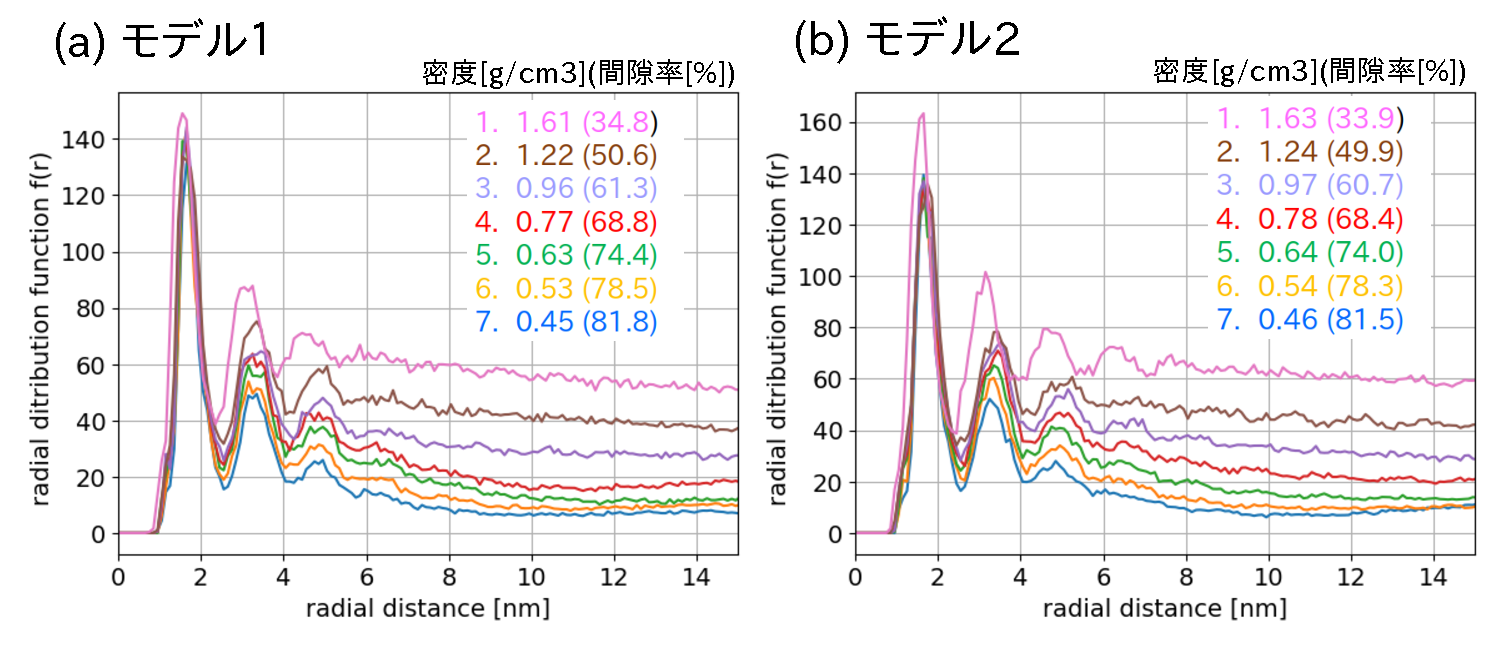
\includegraphics[width=0.5\linewidth]{Figs/fig7.eps} 
	\end{center}
	\caption{
		粗視化粒子の向きを表すために用いる単位接線
		$\hat{\fat{t}}_i,\hat{\fat{t}}_j$
		および, 単位法線ベクトル.
		$\hat{\fat{n}}_i,\hat{\fat{n}}_j$. 
		$\theta_{ij}$は粒子位置$\fat{x}_i$から$\fat{x}_j$を望む方向を,
		$\theta_{ji}$は$\fat{x}_j$から$\fat{x}_i$を望む方向を,
		それぞれの粒子位置における接線ベクトルから測ったときの角度を表す.
	} 
	\label{fig:fig9}
\end{figure}
%--------------------
%\begin{equation}
%	\frac{1}{\sigma_i(\theta_{ij})}
%	=
%	\sqrt{
%		\left( 
%		\frac{\cos\theta_{ij}}{\sigma_0} 
%		\right)^2
%		+
%		\left( \frac{\sin\theta_{ij}}{\sigma_{{\rm sgn}(\theta_{ij})}} \right)^2
%	}
%	\label{eqn:}
%\end{equation}
\section{水和水移動のモデル}
粘土含水系が非平衡状態にあるとき,時間経過に伴い系全体のもつポテンシャルエネルギーが
低下する方向に状態が推移する.従って,系全体のポテンシャルエネルギーが現在の状態よりも
下がる水分の配置をメソMD計算の途上で見つけることができれば,水分移動を考慮しながら,
水和粘土の運動を追跡することができる.メソMD計算における粗視化粒子系全体のエネルギー$E_{tot}$は,各粒子の持つエネルギー$E_i$の総和であるため,
\begin{equation}
	E_{tot}(\fat{\sigma},\fat{V},\fat{X})=\sum_{i=1}^{N}E(i), 
	 \ \ 
	 \left( \fat{\sigma}=\left\{ \sigma^{\pm}_i \right\}
	 ,
	\ \
	 \fat{V}=\left\{ \fat{v}_i\right\}
, \fat{X}=\left\{\fat{x}_i \right\} 
	 \right)
	\label{eqn:Etot}
\end{equation}
と表すことができる.ここで,$\fat{\sigma}$は,全ての粗視粒子の
もつ水分量(系全体での水分分布)を表す$2N$次元のベクトルを,
$\fat{X}$と$\fat{V}$は,粒子系の位置と速度を表す$2N$次元のベクトルである.
式(\ref{eqn:Etot})は,これらを引数に書くことで,全エネルギーが
位置$\fat{X}$,速度$\fat{V}$,水分分布$\fat{\sigma}$に依存する
ことを明示することを意図している.各粗視化粒子のもつエネルギーは,
粘土分子の表面(+面)と裏面(-面)に水和した水分に関連付けられるものの,
2つに分割することができる.すなわち,
\begin{equation}
	E(i)=E^+(i)+E^-(i)
	\label{eqn:sum_Epm}
\end{equation}
と表すことができる.さらに,$E^\pm(i)$は,次のような4つの形態のエネルギーの和
として表すことができる.
\begin{equation}
	E^\pm(i)=E^\pm_{U}(i)+E^\pm_K(i)+E^\pm_{H_2O}(i)+E^\pm_{Surf}(i)
	\label{eqn:Emodes}
\end{equation}
ここに,
$E^{\pm}_U$は,粘土分子間の相互作用力によるポテンシャルエネルギーを,
$E^\pm_K$は運動エネルギーを表す.また,$E^\pm_{H_2O}$は
粘土分子とそれに水和した水分子の相互作用によって生じるポテンシャル
エネルギーを表し,$E^\pm_{Surf}$は水和水の表面自由エネルギーを意味する.
このうち$E^\pm_U(i)$は,異方的LJポテンシャルと式(\ref{eqn:def_thij})を用いて
\begin{equation}
	E_U^\pm(i)=\sum_{j} U(\fat{x}_i,\fat{x}_j)H({\rm sgn}(\pm \theta_{ij}))
	\label{eqn:def_EU}
\end{equation}
によって計算できる.ただし$H(x)$はヘビサイドの単位ステップ関数:
\begin{equation}
	H(x)=\left\{
	\begin{array}{cc}
		1& (x>0)  \\
		0& (x\leq 0) 
	\end{array}
	\right.
	\label{eqn:Step_func}
\end{equation}
である.運動エネルギーは,粒子速度$\fat{v}_i$を用い,
\begin{equation}
	E_K^{\pm}(i)=\frac{1}{2}m^{\pm}(i) |\fat{v}_i|^2 
	\label{eqn:def_EK}
\end{equation}
と書くことができる.ここに,$m^\pm(i)$は,粒子質量$m_i$の分割
\begin{equation}
	m_i=m^+(i)+m^-(i)
	\label{eqn:mi_split}
\end{equation}
を表し,$m^{\pm}$はそれぞれ,$\pm\hat{\fat{n}}_i$側の分子表面に
関連付けることのできる質量を意味する.$m^\pm$は,
無水粘土分子の単位構造が持つ質量を$m_{clay}$, 
水分子1個の質量$m_{H_2O}$,
水和水の分子層数$n^{\pm}$を用いて
\begin{equation}
	m^{\pm}(i)=\frac{m_{clay}}{2}+\frac{3}{2}n_{H_2O}^{\pm}(i)m_{H_2O}
	\label{eqn:def_mpm}
\end{equation}
と書くことができる.なお,$\pm$は着目する粘土分子の面の向きを表し,
係数$3$は,粘土分子単位構造に一層の水分子が水和したときの
単位構造あたりの水分子数である.
水和水と粘土分子の相互作用によるポテンシャルエネルギーに関しては,
水和数$n^\pm_{H_2O}$の関数になると仮定し,
\begin{equation}
	E_{H_2O}^\pm(i)=U_{hyd}
	\left(
		n^\pm_{H_2O}(i)
	\right)
	\label{eqn:def_EH2O}
\end{equation}
と表しておく.$U_{hyd}(n)$は水和数によるエネルギー変化を定める
関数である.粘土分子への水和挙動を$n^\pm$が離散的な値だけをとるとして
モデル化する場合,$U_{hyd}(n)$はデルタ間数列で,
水和数が連続的に変化する場合は,水和数$n$が整数のときに
極小となるような連続関数として与えればよい.本研究では後者のモデルを用いる
ことを検討しているが,後述する数値計算例ではこのエネルギーの変動は考慮していない.
最後に,水分子の表面エネルギーは,気相-水分子相界面の界面自由エネルギー
$\gamma$と,粒子$i$の液相-気相界面$S^\pm_{a/w}(i)$を用いて,
\begin{equation}
	E_{Surf}^{\pm}(i)=\int_{S^\pm_{a/w}(i)}\gamma dS 
	\label{eqn:def_Esurf}
\end{equation}
で与えられる.なお,液相と固相(粘土分子)界面のエネルギーは
$E^\pm_{H_2O}$に含まれると考えておく.
以上のようにして計算される全エネルギーについて,水分分布$\fat{\sigma}$に
関する摂動:
\begin{equation}
	\delta \fat{\sigma}=\left\{ \delta \sigma^\pm_i \right\}
	\label{eqn:var_sig}
\end{equation}
を,全水分量一定:
\begin{equation}
	\sum_{i=1}^N \left( 
		\delta \sigma^+_i
		+
		\delta \sigma^-_i
	\right)
	=0
\end{equation}
の条件において与え,そのときの全エネルギ-$E_{tot}$の変分
\begin{equation}
	\Delta E_{tot}(\fat{\sigma},\fat{V},\fat{X})=
	E_{tot}(\fat{\sigma}+\delta \fat{\sigma},\fat{V},\fat{X})
	-
	E_{tot}(\fat{\sigma},\fat{V},\fat{X})
	\label{eqn:}
\end{equation}
を数値的に計算する.
$\Delta E_{tot}$が負の場合には水分分布を
\begin{equation}
	\fat{\sigma}\rightarrow \fat{\sigma}+\delta \fat{\sigma}
	\label{eqn:sig_update}
\end{equation}
と更新する.運動方程式を数値的に積分する際の適当な時間ステップにおいて,
このような規則に従い水分分布を変更することで,水和粘土分子の運動と変形
だけでなく,粘土分子と水和水の相対的な運動(水和水移動)のシミュレーション
を行うことができる.
%%%%%%%%%%%%%%%%%%%%%%%%%%%%%%%%%%%%%%%%%%%%%%%%%%%%%
\section{数値解析例}
\subsection{水分移動を伴わない場合}
図\ref{fig:fig1}に示すような,200nm$\times$200nmのユニットセルに40個の
粘土分子をもつ粗視化MDモデルを考え,周期境界条件のもと,
一定のひずみ速度で60\%等方的に圧縮する場合を例として数値シミュレーションの
結果を示す.図\ref{fig:fig1}の左は,その際に用いた粘土分子の初期配置を示したもので,
この図の右側には,粘土分子幅の度数分布がヒストグラムとして示されている.
その他,数値シミュレーションに関する主要な計算条件を以下に示す.
\begin{itemize}
\item
ユニットセルサイズ:200$\times$200[nm$^2$]
\item
粘土分子数:M=40,\, 粗視化粒子数:N=2,000
\item
時間ステップ長:$\Delta t=$0.2[ps], 時間ステップ数:50,000ステップ
\item
特性距離:$\sigma^\pm=$1.5[nm](2層膨潤),$\sigma^0=$1.35[nm]
\end{itemize}
第1の数値解析例では,全ての粘土分子表面に水分子が2層水和分だけ水和された状態から
計算をスタートし,圧縮の過程においても,粘土分子の各点に水和した水分の量は一定
としている.図\ref{fig:fig2}は,この場合の結果をスナップショットとして示したもので,
(a)から(f)の順に時間が経過し,ユニットセルのサイズが小さくなっている.
なお,(a)は圧縮開始から80[ps]が経過したときの結果を示し,(f)は1[ns]経過して圧縮が
終了した時点の粘土分子の様子を示している.この図に示されるように,当初分散していた
粘土分子が,ユニットセルの圧縮にともない次第に積層し,粘土層間の他にも
大きな空洞部分ができる様子が見られる.このシミュレーション結果は水分が移動は無く,
従来の粗視化メソMDによる結果と大きく変わるところは無い.ただし,LJポテンシャルは
縦方向と横方向の特性距離$\sigma^\pm$と$\sigma^0$が異なる異方的なものを用いている.
------------------
\begin{figure}[h]
	\begin{center}
	\includegraphics[width=1.0\linewidth]{Figs/model.eps} 
	\end{center}
	\caption{
		粘土分子の初期状態と分子幅の分布(水分量が2層膨潤状態相当で
		均一かつ一定の場合).
	} 
	\label{fig:fig1}
\end{figure}
%--------------------
%--------------------
\begin{figure}[h]
	\begin{center}
	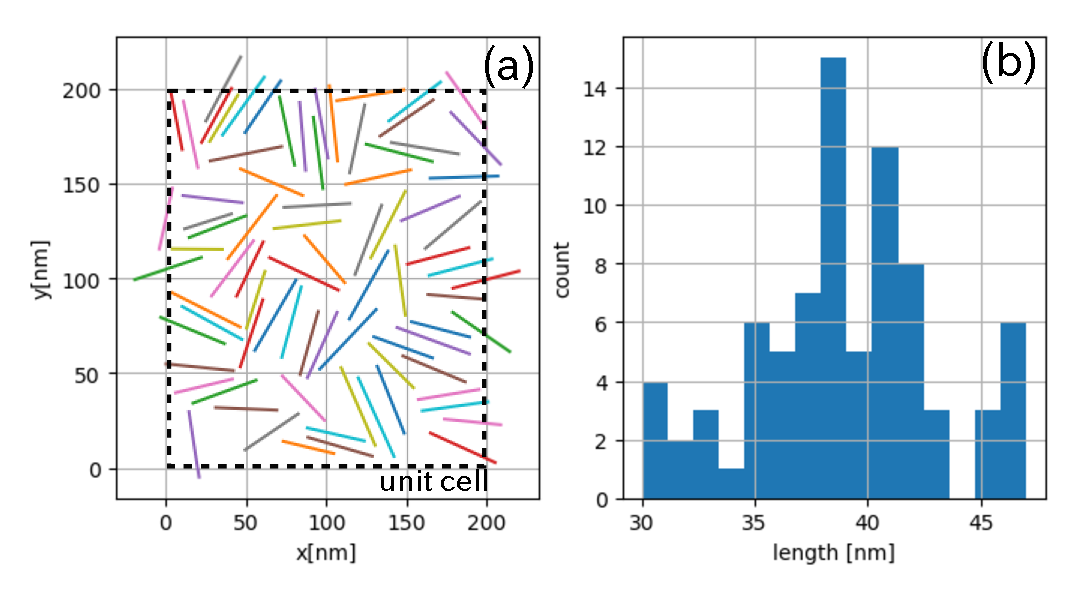
\includegraphics[width=0.9\linewidth]{Figs/fig1.eps} 
	\end{center}
	\caption{
		粘土含水系モデルを等方的に圧縮したときの挙動.水分移動を伴わない場合($\sigma^\pm=1.5$[nm]).
	} 
	\label{fig:fig2}
\end{figure}
%--------------------
\subsection{水分移動を伴う場合}
次に,図\ref{fig:fig1}に示したモデルを用い,水分移動を考慮して行った圧縮凝集
挙動のシミュレーション結果を示す.この計算例では,ランダムに選択した2つの
粗視化粒子の間で水分のやり取りが発生するか否かを,運動方程式の計算スッテップ毎に
粒子数の回数だけ行っている.ただし,1計算ステップでの水分の変化は,
分子間相互作用ポテンシャルの特性距離$\sigma_i^\pm$を$\pm 0.03$[nm]だけ変化させることで行っており,
これは水分子層の1/5の厚さに相当する.また,水分の移動は
\begin{equation}
	\left| \fat{x}_i -\fat{x}_j\right| < 3.5 \bar{\sigma}(i,j)
	\label{eqn:rij_max}
\end{equation}
の条件を満たす粒子$i$と$j$の間でのみ起きると仮定している.
図\ref{fig:fig3}は,以上の条件による計算結果を示したもので,(a)から(f)
の順に時間が経過している.なお,各々のスナップショットに対する
圧縮開始からの経過時間は,図\ref{fig:fig2}と同じである.
水分の移動を考慮した場合も,分散状態にあった粘土分子は次第に積層構造を作り,
圧縮の進展につれ徐々に明確かつ大きな間隙が発生する.また,(a)から(c)までの
時間では,水分の移動を考慮しない場合と非常によく似た結果が得られているが,
後半の(d)から(f)の時間帯では,水分移動を考慮した場合の方が積層数が小さく,
積層した分子の集団がより屈曲していることが分かる.(f)に示した結果は,
シミュレーションの最終段階で圧縮を終了させた時点の結果だが,
計算を継続した場合はこの後も系は緩和を続け,粘土や水分配置は変化する.
しかしながら,水分移動を考慮した場合としない場合の結果は,シミュレーションの
終了時点で明らかに異なり,最終的に安定な状態に至った段階でも大きくことなる
組織構造をとる可能性が高い.
%--------------------
\begin{figure}[h]
	\begin{center}
	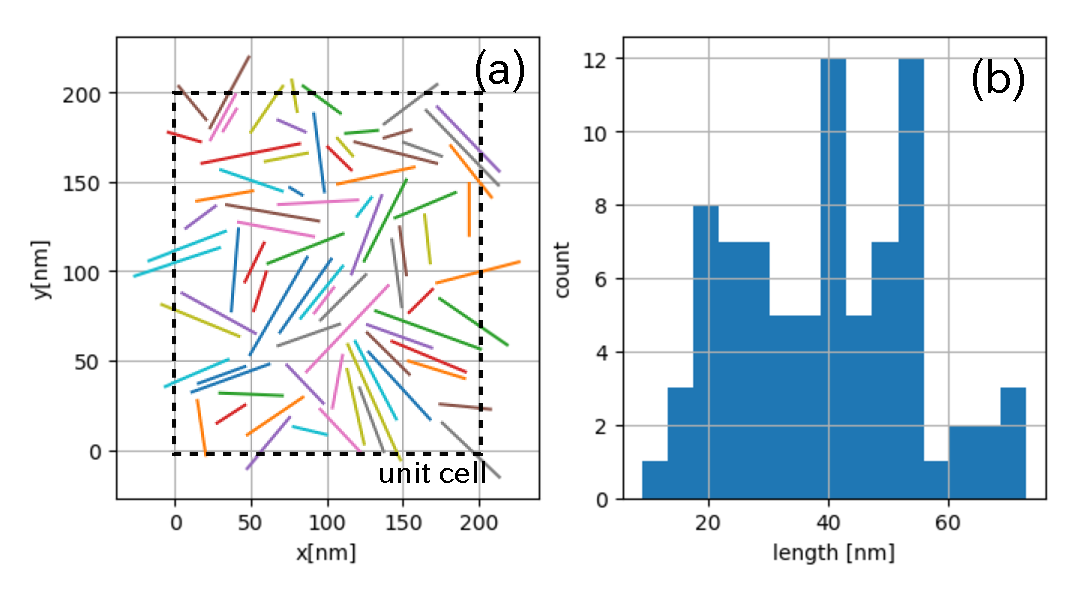
\includegraphics[width=0.9\linewidth]{Figs/fig2.eps} 
	\end{center}
	\caption{
		粘土含水系モデルを等方的に圧縮したときの挙動.
		水分移動を伴う場合($\sigma^\pm=1.5$[nm]から計算を開始).
	} 
	\label{fig:fig3}
\end{figure}
%--------------------
\subsection{不均一な初期水分分布をもつ系の圧縮}
粘土分子が分散した状態では,それぞれの分子が異なる量の水和水を持つ状況が
起きると想定する必要がある.その極端なケースとしてここでは,初期状態において
半数の粘土分子が無水の状態にあり,残る半数が3層膨潤状態に相当する水分を持つとして
行った,圧縮凝集シミュレーションの結果を示す.図\ref{fig:fig8}はこのときの,
初期粘土分子の配置を示したものである.分子数はこれまで同様$M=$40としているが,
初期状態での特性距離$\sigma^\pm$が分子によって異なるため,初期状態で
粘土分子間に相互作用が生じないよう、分子サイズや初期配置は前述のモデルと
若干異なるものを用いている.この場合の系の時間的変化を図\ref{fig:fig4}に示す.
初期配置や分子サイズがこれまでの例と異なることには注意が必要であるが,
(d)に示した時間帯から,粘土分子は小さなクラスターを作りはじめ,圧縮終了時点(f)では,
これまでに示した計算例よりも屈曲が大きく,より小さな多数の空洞が形成されている.
このことは,粘土含水系を圧縮凝集させたとき,初期水分配置が,最終的に形成
される積層構造の積層数や層外の間隙サイズに影響することを示唆している.
%--------------
\begin{figure}[h]
	\begin{center}
	\includegraphics[width=1.0\linewidth]{Figs/model2.eps}
	\end{center}
	\caption{
		粘土分子の初期状態と分子幅の分布
		(水分量が0層あるいは3層膨潤状態相当の粘土分子が同数ずつ存在する場合).
	}
	\label{fig:fig8}
\end{figure}
%--------------------
%--------------------
\begin{figure}[h]
	\begin{center}
	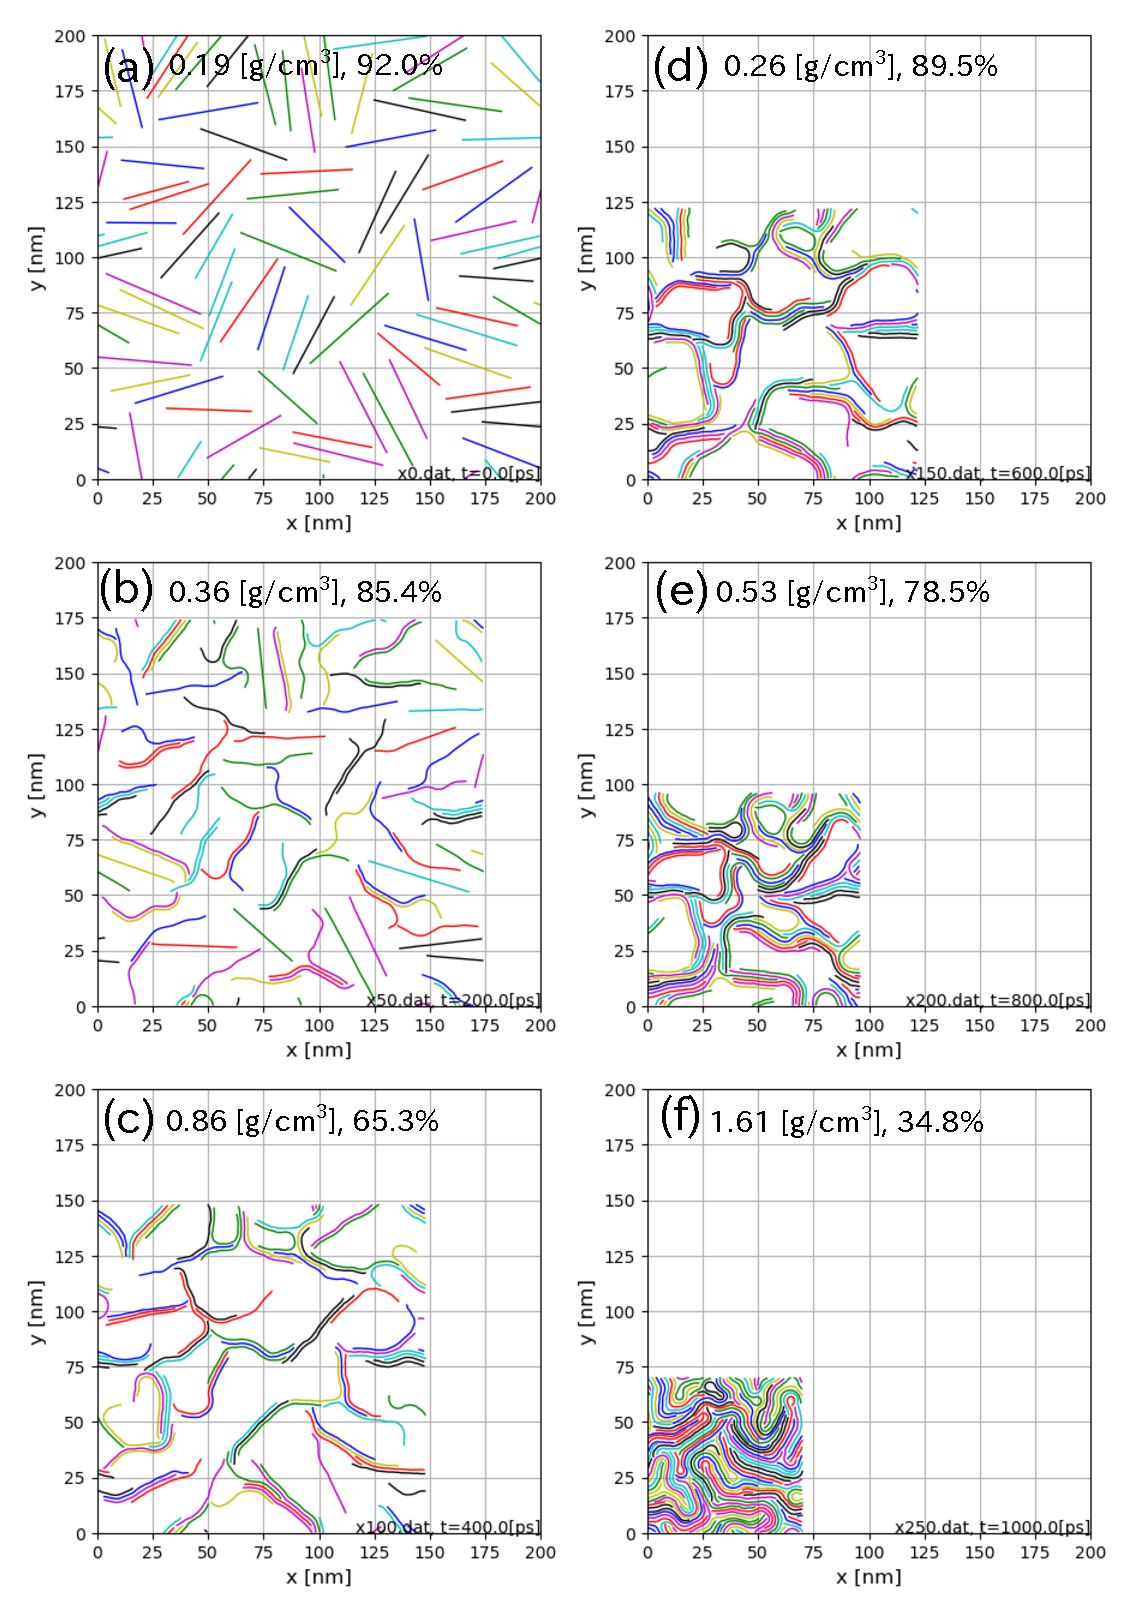
\includegraphics[width=0.9\linewidth]{Figs/fig3.eps} 
	\end{center}
	\caption{
		粘土含水系モデルを等方的に圧縮したときの挙動.
		水分移動を伴う場合(初期状態において$\sigma^\pm=0.9$と$1.8$[nm]の
		分子が同数ずつの場合).
	} 
	\label{fig:fig4}
\end{figure}
%--------------------
\subsection{水分分布状況の可視化}
最後に,水分の分布状況を可視化した結果をこれまでの3つの計算ケースそれぞれに
ついて図\ref{fig:fig5}から図\ref{fig:fig7}に示す.おのおの図において,
(a)は圧縮開始から$t=$720[ps]経過した時点の,(b)は圧縮終了時($t=$1[ns]経過時)の
様子を示している.水分移動を考慮していない図\ref{fig:fig5}の結果では,
水分が粘土分子表面に均一に固定的に分布しているため,粘土層間の距離が一様でない
部分では細かな空隙が残っていることが分かる.一方,水分移動を考慮した図\ref{fig:fig6}と
図\ref{fig:fig7}の結果では,積層した粘土の層間には水分が浸透して空隙はほとんど残されていない.
ただし,初期の水分分布状態が異なる図\ref{fig:fig6}と図\ref{fig:fig7}の結果を比べると,
図\ref{fig:fig7}の方が,より水分分布の空間的な変動が大きい.
このことは,圧縮の進行速度に対し,粘土分子が積層構造を発達させるために
必要な水分を移動させる時間を図\ref{fig:fig7}のケースでは
十分に確保することができず、その結果より小さな多数の空洞が残たまま
圧縮が進むことを意味している.
%--------------------
\begin{figure}[h]
	\begin{center}
	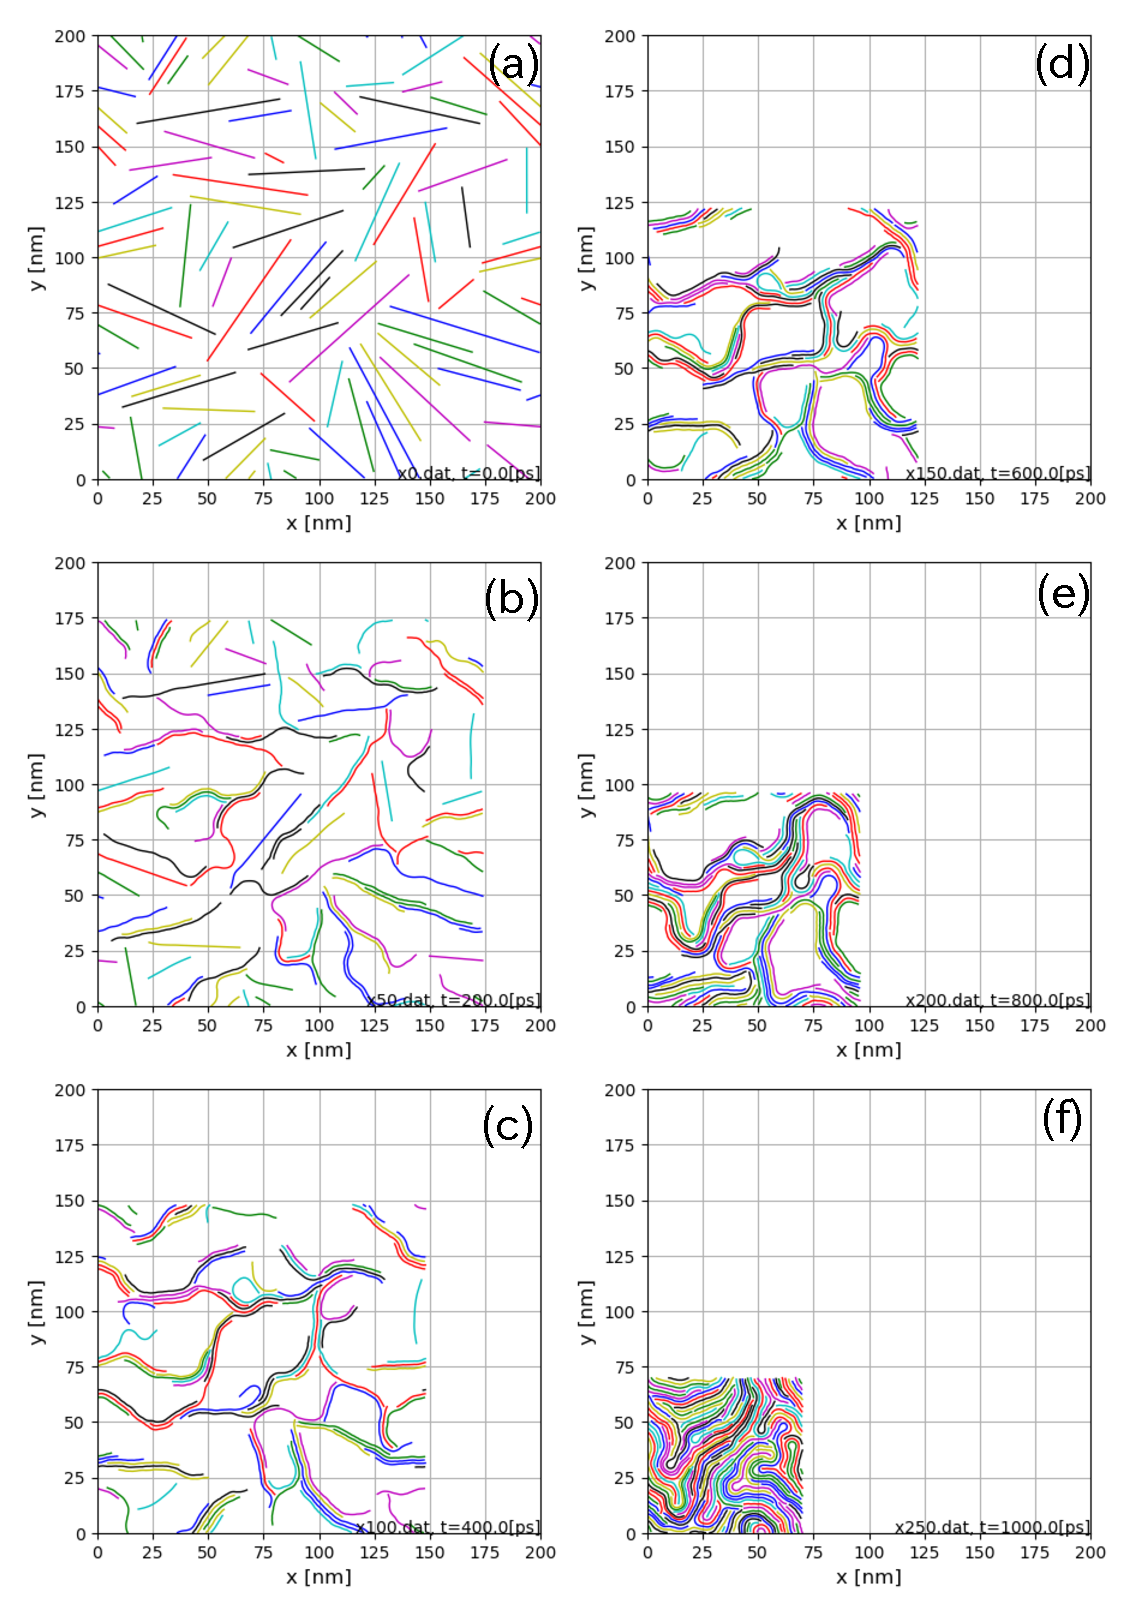
\includegraphics[width=0.8\linewidth]{Figs/fig4.eps} 
	\end{center}
	\caption{
		粘土分子と水分の分布状況($\sigma^\pm=1.5$[nm],水分移動を伴わない場合).
	} 
	\label{fig:fig5}
\end{figure}
%--------------------
%--------------------
\begin{figure}[h]
	\begin{center}
	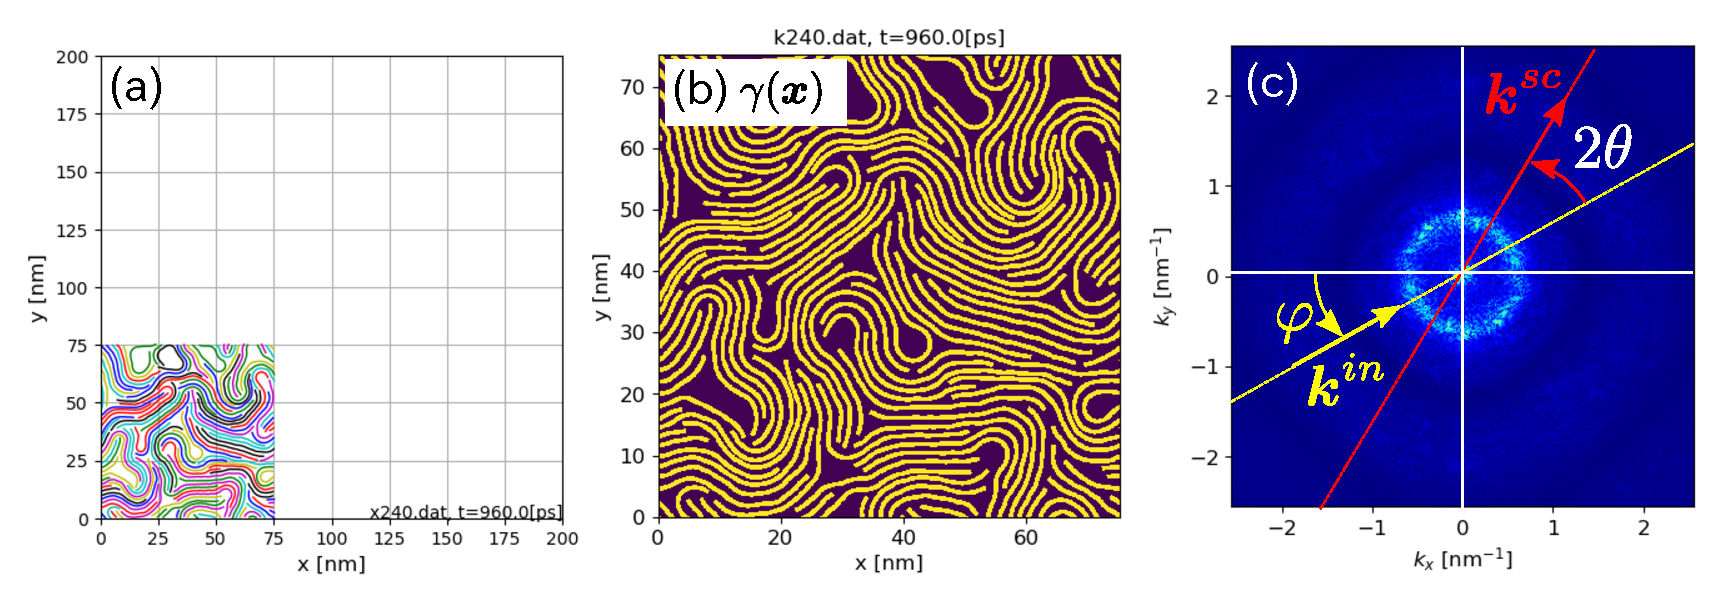
\includegraphics[width=0.8\linewidth]{Figs/fig5.eps} 
	\end{center}
	\caption{
		粘土分子と水分の分布状況(初期状態において$\sigma^\pm=1.5$[nm],
		水分の移動を考慮した場合).
	} 
	\label{fig:fig6}
\end{figure}
%--------------------
%--------------------
\begin{figure}[h]
	\begin{center}
	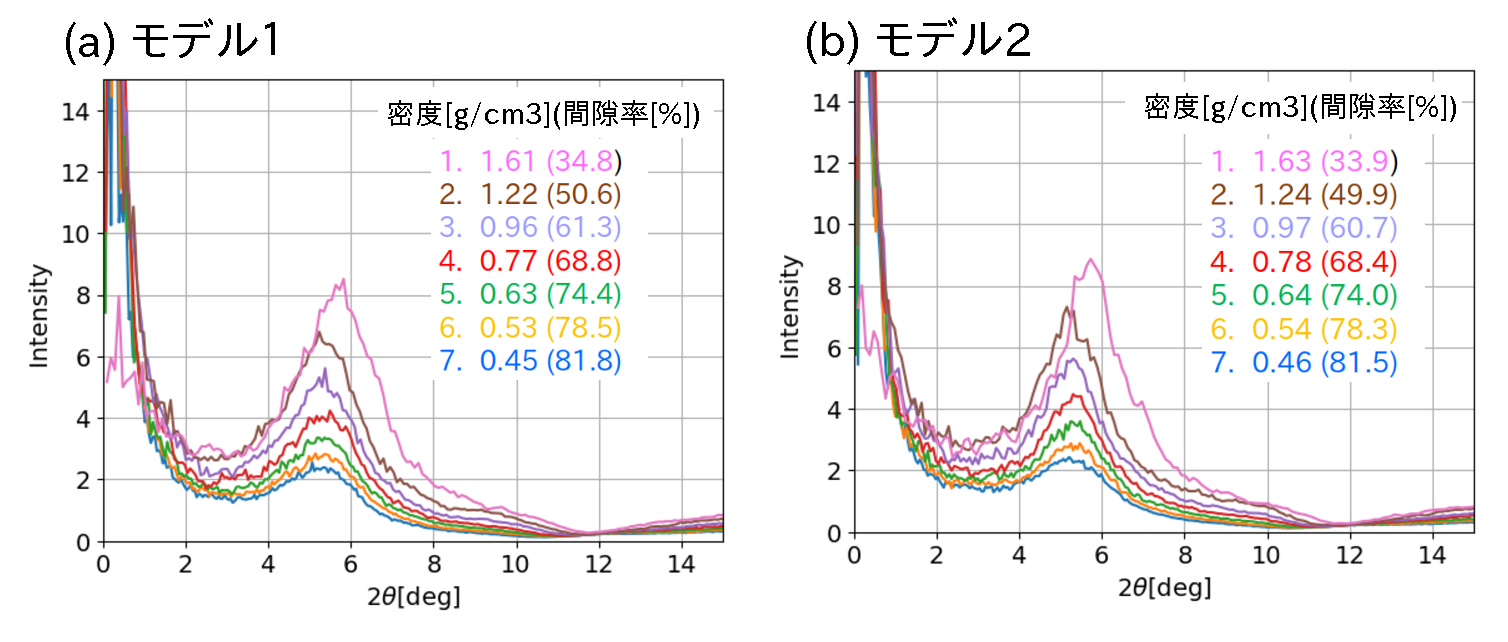
\includegraphics[width=0.8\linewidth]{Figs/fig6.eps} 
	\end{center}
	\caption{
		粘土分子と水分の分布状況(初期状態において$\sigma^\pm=0.9$と1.8[nm]の
		粘土分子が同数存在し,水分移動を考慮した場合).
	} 
	\label{fig:fig7}
\end{figure}
%--------------------
\section{まとめ}
本年度の研究では,粘土含水系のメソMDシミュレーションにおいて水和水の移動を考慮する
ための必要となるシミュレーション手法を開発し,以下の成果を得た.
\begin{itemize}
\item
不均一な水和水分布を表現するために,異方的なLenard-Jones型分子間力ポテンシャルを開発した.
これにより粘土分子の表裏面を区別するとともに,位置によって異なる水和水の分布を考慮することが
可能となった.
\item
粗視化メソMDにおいて水分移動を考慮する方法として
水分分布の変化に伴うポテンシャルエネルギーの増減を基準として利用する方法を提案した.
この方法では,粘土分子の集合状態や層間の膨潤状態(水分量の多寡),液相表面の形状
の影響を考慮して水分の移動を行うことができる.本年度は,これら影響因子のうち,
特に,粘土分子の相互作用に起因した水分移動を考慮できるシミュレーションを実現した.
\item
以上の方法をメソMDプログラムにおいて実装し,粘土含水系の圧縮凝集シミュレーションを行った.
数値シミュレーションの結果を用い,水分移動を行う場合,行わない場合の比較や
初期水分状態が均一な場合と不均一な場合の比較を行った.
\item
一連の数値シミュレーションの結果から,水分移動を考慮することで,積層した粘土層間に小さな気泡が
残ることの無いより妥当な結果が得られるようになることがわかった.また,初期水分分布に偏りが
ある場合,比較的屈曲の大きな粘土分子の積層構造が形成され,積層構造外の空隙部はあまり大きく
ならないことが分かった.
\item
数値シミュレーションの結果として得られたこれらの知見は,粘土含水系の現実的な組織構造を
再現するためには,水分の移動を考慮することが必要でことを示唆していると考えられる.
\end{itemize}
本年度の研究では,水分移動に関して,粘土分子間の相互作用エネルギー$E_U$のみを考慮している.
そのため,より現実的な組織構造モデルを得るためには,粘土分子と水分子の相互作用エネルギー
$E_{H_2O}$や,液相の界面自由エネルギー$E_{Surf}$も考慮したシミュレーションを行うことが
今後の課題となる.そのためには,$E_{H_2O}$や$E_{Surf}$を分子動力学計算を用いて定量的に
求める必要がある.また,水分移動の頻度や量を,物理化学的な根拠をもって定量的に与えることも
分子動力学計算を援用して取り組むべき重要な課題の一つと言える.最後に,粘土含水系モデルと
シミュレーション結果の妥当性を検証するには,弾性係数や電気化学インピーダンスをはじめとする,
実験で観測できるマクロ物性値との比較を行うことも重要である.
\end{document}


